\documentclass[../main.tex]{subfiles}

\graphicspath{{\subfix{../images/}}}

\begin{document}

\section{Task 3}

Write a C-application that implements a command language interpreter, controlled via the USB-UART interface. The following commands must be implemented:

\begin{itemize}
    \item \textbf{1 -} Sets tthe binary value from 0-15 on the red led's by reading switch input (SW0-SW3).
    \item \textbf{2 -} Counts binary the redd led's using a timer of 1 sec.
\end{itemize}

\subsection*{Solution}

We will start off by describing the system in general: how we will handle timing, UART communication, etc.. UART communication is simple when using \texttt{inbyte()}, which is a wrapper for \texttt{XUartPs\_RecvByte()}, defined in \texttt{xuartps\_hw.h}. Identifying the function in the header, we read that:

\begin{enumerate}
    \item \texttt{XUartPs\_RecvByte()} receives a byte from the device.
    \item \texttt{XUartPs\_RecvByte()} operates in polled mode and blocks until a byte has been received.
\end{enumerate}

Especially point 2 is important. We ideally want to be reading the UART constantly so the user can switch applications during runtime, but since \texttt{inbyte()} blocks until a byte is received, it is not sufficient with just use a "\textit{Arduino-style}" \texttt{while(1)} loop. Instead, we will use dynamic interrupt handling. To do this we will use the \texttt{XScuTimer} and \texttt{XScuGic} (General Interrupt Controller) drivers. The \texttt{XScuTimer} will be used to generate an interrupt every X second(s), and the \texttt{XScuGic} will be used to handle the interrupt.

\begin{myminted}{main.c - Initialization}
    int main (void) 
    {
        GpioInit(&DipInstance, XPAR_SWITCHES_DEVICE_ID);
        GpioInit(&PushInstance, XPAR_BUTTONS_DEVICE_ID);
    
        ScuTimerInit(&TimerInstance, XPAR_XSCUTIMER_0_DEVICE_ID, 100*MILLISECOND);
        ScuIntrInit(&IntcInstance, XPAR_SCUGIC_SINGLE_DEVICE_ID);
        TimerSetupIntr(&IntcInstance, &TimerInstance, XPAR_SCUTIMER_INTR);
    
        int input;
    
        xil_printf("\r\n-- Start of the Program --\r\n");
    
        while (1)
        {
        ...
        ...
        ...
        }
    }
\end{myminted}

\newpage

The functions \texttt{ScuTimerInit()}, \texttt{ScuIntrInit()} and \texttt{TimerSetupIntr()} enables the timer, binds the interrupt controller, and sets the timer to trigger an interrupt every 100 ms. The 100 ms is just a default value. Each application will be able to configure the timer accordingly by using the wrapper functions \texttt{TimerLoad()}, \texttt{TimerStart()} and \texttt{TimerStop()}.

\begin{myminted}{main.c - Timer Functions}
void TimerStart(XScuTimer *TimerInstancePtr)
{
    XScuTimer_Start(TimerInstancePtr);
}

void TimerStop(XScuTimer *TimerInstancePtr)
{
    XScuTimer_Stop(TimerInstancePtr);
}

void TimerLoad(XScuTimer *TimerInstancePtr, u32 TimerCounter)
{
    XScuTimer_LoadTimer(TimerInstancePtr, TimerCounter);
}
\end{myminted}

A pointer \texttt{*TimerFunctionPtr}, defined in the global scope, will be used in the interrupt handler. This pointer will be set to the function that should be called when the timer interrupt is triggered. The function will be set in the main loop, depending on the user input. The interrupt handler will then call the function pointed to by \texttt{*TimerFunctionPtr}.

\begin{myminted}{main.c - TimerIntrHandler()}
static void TimerIntrHandler(void *CallBackRef)
{
    XScuTimer *TimerInstancePtr = (XScuTimer *) CallBackRef;
    XScuTimer_ClearInterruptStatus(TimerInstancePtr);

    if (TimerFunctionPtr != NULL) {
        TimerFunctionPtr();
    }
}
\end{myminted}

All devices necessary are now intialized. In the main loop we will wait for UART input, using \texttt{inbyte()}, and enter the corresponding application in a \texttt{switch}-statement. The procedure is roughly as follows:

\begin{enumerate}
    \item Wait for UART input.
    \item Parse input and enter corresponding application (switch-statement).
    \item Stop the timer and set the function pointer to the application.
    \item Load the timer counter register.
    \item Start the timer.
\end{enumerate}

\newpage

\begin{myminted}{main.c - Main Loop}
while (1)
{
    xil_printf("\r\nCMD:> ");
    input = inbyte();
    xil_printf("%c", input);
    switch (input)
    {
        case '0':
            xil_printf("\r\nNo action.");
            xil_printf("\r\nStopping Timer Routine.\n");
            TimerStop(&TimerInstance);
            TimerFunctionPtr = NULL;
            break;
        case '1':
            xil_printf("\r\nStarting Program 1.");
            xil_printf("\r\nSwitches to LEDs.\n");
            TimerStop(&TimerInstance);
            TimerFunctionPtr = &read_switches;
            TimerLoad(&TimerInstance, 100*MILLISECOND);
            TimerStart(&TimerInstance);
            break;
        case '2':
            xil_printf("\r\nStarting Program 2.");
            xil_printf("\r\nLED Binary Counting.\n");
            TimerStop(&TimerInstance);
            TimerFunctionPtr = &count_leds;
            TimerLoad(&TimerInstance, 1000*MILLISECOND);
            TimerStart(&TimerInstance);
            break;
        default:
            xil_printf("\r\nUnrecognized input. \"%c\"", input);
            break;
    }
}
\end{myminted}

The actual applications are simple void functions. The \texttt{read\_switches()} function is triggered every 100 ms and reads the switches, setting the LEDs accordingly.

\begin{myminted}{main.c - read\_switches()}
void read_switches()
{
	int switch_read = XGpio_DiscreteRead(&DipInstance, 1);
	LED_IP_mWriteReg(XPAR_LED_IP_S_AXI_BASEADDR, 0, switch_read);
}
\end{myminted}

\newpage

The \texttt{count\_leds()} function is triggered every second and increments a \texttt{static} counter variable, displaying the binary value on the LEDs.
\begin{myminted}{main.c - count\_leds()}
void count_leds()
{
	static u8 count = 0;
	count = (count + 1) & 0x0F;
	LED_IP_mWriteReg(XPAR_LED_IP_S_AXI_BASEADDR, 0, count);
}
\end{myminted}

The command interpreter is now complete. The full code can be found on our GitHub repository. The UART communication is done using PuTTY, as shown in the screenshot below.

\begin{figure}[h]
    \centering
    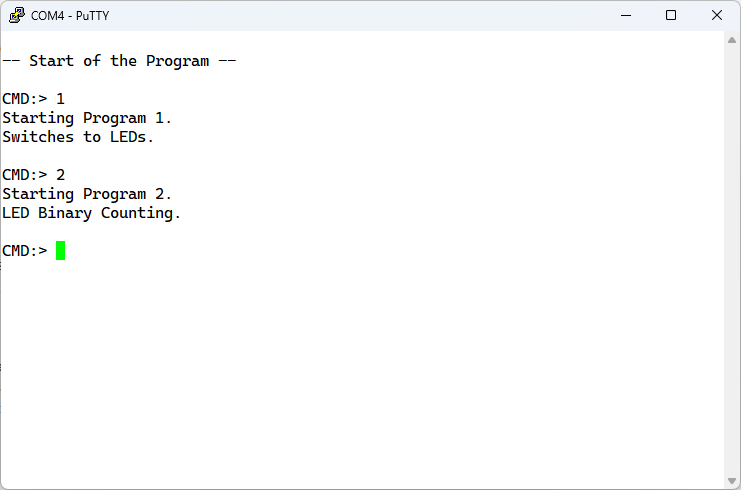
\includegraphics[width=1\textwidth]{task3_putty.png}
\end{figure}

\end{document}